%%%%%%%%%%%%%%%%%%%%%%% file typeinst.tex %%%%%%%%%%%%%%%%%%%%%%%%%
%
% This is the LaTeX source for the instructions to authors using
% the LaTeX document class 'llncs.cls' for contributions to
% the Lecture Notes in Computer Sciences series.
% http://www.springer.com/lncs       Springer Heidelberg 2006/05/04
%
% It may be used as a template for your own input - copy it
% to a new file with a new name and use it as the basis
% for your article.
%
% NB: the document class 'llncs' has its own and detailed documentation, see
% ftp://ftp.springer.de/data/pubftp/pub/tex/latex/llncs/latex2e/llncsdoc.pdf
%
%%%%%%%%%%%%%%%%%%%%%%%%%%%%%%%%%%%%%%%%%%%%%%%%%%%%%%%%%%%%%%%%%%%

\documentclass[runningheads,a4paper]{llncs}

\usepackage[utf8]{inputenc}
\usepackage{amsmath}
\usepackage{algorithm}
%\usepackage{cite}
\usepackage{natbib}
\usepackage[noend]{algpseudocode}
\renewcommand{\algorithmicforall}{\textbf{for each}}

\newcommand{\var}[1]{\mathit{#1}}
\newcommand{\func}[1]{\mathrm{#1}}

\algdef{SE}[DOWHILE]{Do}{doWhile}{\algorithmicdo}[1]{\algorithmicwhile\ #1}%

\usepackage{natbib}
\bibliographystyle{apalike-fr}

\usepackage{amssymb}
\setcounter{tocdepth}{3}
\usepackage{graphicx}

\usepackage[french]{babel} % Pour adopter les règles de typographie française
\usepackage[T1]{fontenc} % Pour que les lettres accentuées soient reconnues

\usepackage{url}

\urldef{\mailsa}\path|{alfred.hofmann, ursula.barth, ingrid.haas, frank.holzwarth,|
\urldef{\mailsb}\path|anna.kramer, leonie.kunz, christine.reiss, nicole.sator,|
\urldef{\mailsc}\path|erika.siebert-cole, peter.strasser, lncs}@springer.com|    
\newcommand{\keywords}[1]{\par\addvspace\baselineskip
\noindent\keywordname\enspace\ignorespaces#1}

\begin{document}

\mainmatter 

\title{Model Checking CTL}

\titlerunning{Model Cheking CTL}

\author{PAQUET Michaël}

\institute{Université Libre de Bruxelles}

\authorrunning{PAQUET Michaël}

\toctitle{Résumé}
\tocauthor{{}}

\maketitle

\begin{abstract}
Le "model-checking" est une technique générale de "vérification automatique de systèmes informatiques". Elle permet donc de prouver, de façon automatique (à l'aide d'un algorithme) qu'un système est correct … ou de détecter des bugs. Au cours de notre rapport, nous allons donc expliquer de manière plus détaillée ce qu'est le model-checking CTL et comment celui-ci fonctionne d'un point de vue algorithmique. Ensuite, nous vérifierons via une implémentation qui nous est propre le fonctionnement de ce modèle. 
\end{abstract}

\medskip

\begingroup
\let\clearpage\relax
\tableofcontents
\addcontentsline{toc}{section}{Introduction}
\endgroup

\medskip
\medskip

\newpage 

\section*{Introduction}

Avec l'évolution technologique faisant acte de présence jours après jours, la plupart des services, informatique ou non, sont maintenant gérés via des système informatiques vérifiant leur bon fonctionnement. Mais pour certains services, il est impératif que ces systèmes fonctionnent correctement.\\


\noindent Prenons l'exemple d'une voie ferrée. Dans ce cas de figure-ci, il est impératif que les portes soient fermées lorsque le train traverse le passage à niveau. Comme dit précédemment, un système informatique s'occupera de gérer cela.

\noindent Mais puisqu'on ne peut pas se permettre la moindre erreur, nous nous devons de vérifier que le système n'échouera jamais, et c'est dans ce cas de figure que le \textit{Model Checking} fut créé et utilisé.\\

\noindent Au cours de l'explication de ce qu'est le model checking CTL, nous passerons donc en revue chacun des points de vue qu'on peut adopter lorsqu'on parle de \textit{Model Checking CTL}.\\
Le premier point que nous aborderons sera l'aspect analytique du modèle (Qu'est-ce qu'on doit vérifier ?). Lors de ce chapitre, nous allons montrer la façon dont on découpe un système pour en faire des structures propice à l'analyse et à la vérification. Des structures comme les \textit{Kripke models} ou encore les arbre seront bien évidemment abordées. Une fois ces objets observés, nous étudierons la façon dont on peut vérifier l'efficacité d'un système.


\section{Chapitre 1}
\subsection{Du graphe aux arbres de recherche}

Pour pouvoir analyser un système et pouvoir vérifier son efficacité, il est utile de le dériver en un graphe. Afin d'imager nos propos, reprenons l'exemple de la voie ferrée :\\ imaginons donc une voie ferrée sur laquelle aucun train ne circule. La voie est donc vide. On peut constate là un premier état de notre voie ferrée, l'état \textbf{vide}. Lorsque notre voie est vide, il se peut qu'à tout moment, un train soit \textbf{en approche}, et qu'on doive commencer à fermer les portes. Après quoi la voie sera \textbf{occupée} par le train pour qu'ensuite celui-ci reparte et laisse la voie \textbf{vide}.\\

\noindent Un tel système peut être représenté sous la forme vue sur la figure  \ref{label-image3}.

\begin{figure}[!h]
	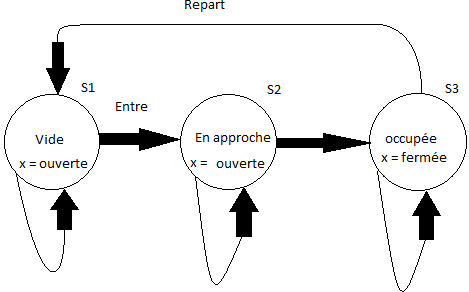
\includegraphics[scale=0.5]{graphe.png}
	\centering
	\caption{Modèle Kripke}
	\label{label-image3}
\end{figure}

\noindent Avec x étant une variable propositionnelle pour déterminer l'état des portes.\\
Un tel modèle est appelé \textit{Kripke Model}.\\
Par convention, le modèle \textit{Kripke} : $$K = (V, S, S_{0}, I, R)$$ \\
est le modèle \textit{Kripke} dont :
\begin{enumerate}
\item \textbf{V}\{ouverte, se ferme, fermée\} est un ensemble fini de propositions atomiques.
\item \textbf{S}\{vide, en approche, occupée\} est en ensemble fini d'état.
\item \textbf{$\textrm{S}_\textrm{0}$} est l'état initial.
\item \textbf{I : S $\rightarrow$ 2\up{V}} est la fonction qui lie chaque états avec les propositions qui y sont liées.
\item \textbf{R} est l'ensemble des relations entre chacun des états.
\end{enumerate}

\begin{figure}[!h]
	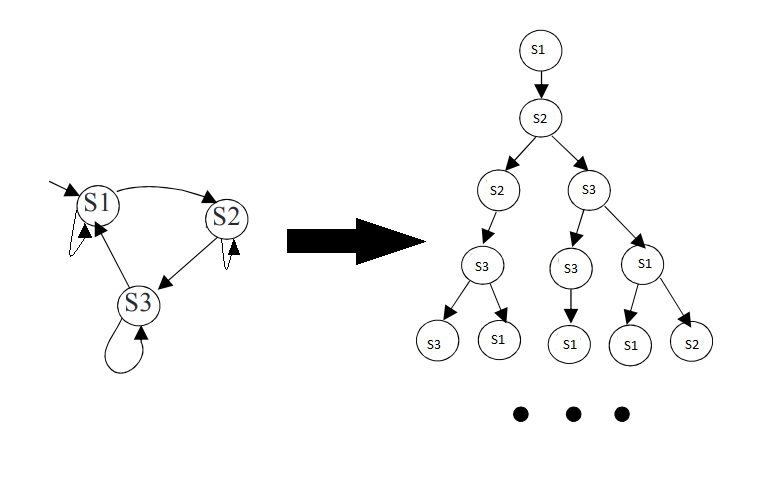
\includegraphics[scale=0.4]{kripke.png}
	\centering
	\caption{du Modèle Kripke à l'arbre de recherche}
	\label{label-image4}
\end{figure}

\noindent Nous avons donc un graphe cyclique dont le nombre d'états est fini. Il est intéressant de voir que lorsque l'on créer un arbre sur base d'un tel graphe, celui-ci sera infini dû au carractère cyclique du graphe. Nous pouvons voir ce que donne la création d'un arbre sur base de modèle Kripke sur la figure \ref{label-image4}.



\noindent C'est maintenant grâce à de telles structures que nous allons pouvoir analyser notre système et vérifier que celui-ci soit infaillible.

\subsection{Computational Tree Logic (CTL)}

La syntaxe de la \textit{Computational Tree Logic} utilise des formule booléennes : \textit{True} et \textit{False} sont donc des formules \textit{CTL}.\\
Les variables propositionnelles sont des formules \textit{CTL}.\\
Ainsi, si $\varphi$ et $\psi$ sont des formules \textit{CTL} alors : $\lnot \varphi$, $\varphi \land \psi$ et $\varphi \lor \psi$ le sont aussi.\\

\noindent En plus de cela, plusieurs opérations sont également des formules \textit{CTL} : 

\begin{itemize}
\item EX $\varphi$ : $\varphi$ apparait dans un des états suivants.
\item EF $\varphi$ : Dans au moins un chemin, $\varphi$ apparait dans un état future.
\item EG $\varphi$ : Dans au moins un chemin, $\varphi$ apparait dans tous les états futures.
\item E[$\varphi \cup \psi$] : Dans au moins un chemin, $\varphi$ apparait jusqu'à ce que $\psi$ apparaisse. \\
\end{itemize}


\noindent Les opérations ici citées sont à chaque fois des "\textit{There exists}" (EX = Exists next), mais il existe également les opérations "\textit{ForAll}". \\
Ainsi, AX $\varphi$ : $\varphi$ apparait dans \textbf{tous} les états suivants.
AF, AG, A$\cup$ sont donc aussi des opérations valables.\\

\noindent Voici à titre d'exemple un schéma pour se donner une idée de ce que ces opérations signifient.

\begin{figure}[!h]
	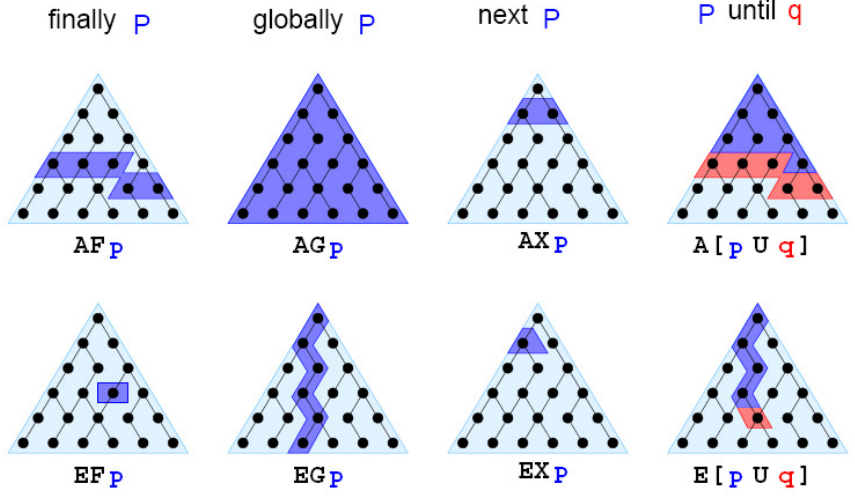
\includegraphics[scale=0.4]{liveness.png}
	\centering
	\caption{Exemple}
	\label{label-image5}
\end{figure}


\noindent De ces opérateurs découlent plusieurs propriétés. En voici une liste non exhaustive : 
\begin{itemize}
\item $\lnot$ AX $\varphi \Leftrightarrow $ EX $\lnot \varphi$
\item $\lnot$ AF $\varphi \Leftrightarrow $ EG $\lnot \varphi$
\item AF $\varphi \Leftrightarrow $ A[true $\cup \ \varphi$]
\item AG $\varphi \Leftrightarrow \varphi \ \land$ AX AG $\varphi$
\item AF $\varphi \Leftrightarrow \varphi \ \lor$ AX AF $\varphi$
\item A[false $\cup \ \varphi$] $ \Leftrightarrow $ E[false $\cup \ \varphi$] = $\varphi$
\item A[$\varphi \ \cup \ \psi$] $ \Leftrightarrow \psi \ \lor$ ($\varphi \ \land$ AX A[$\varphi \ \cup \ \psi$])
\item E[$\varphi \ \cup \ \psi$] $ \Leftrightarrow \psi \ \lor$ ($\varphi \ \land$ EX E[$\varphi \ \cup \ \psi$])
\item A[$\varphi$ W $\psi$] $ \Leftrightarrow \lnot$ E[$\lnot \psi \ \cup$ ($\lnot \varphi \ \land \ \lnot \psi$)]\\
\end{itemize}

\noindent Maintenant que nous avons fait un tour non exhaustif de ce qu'était la syntaxe de \textit{CTL}, abordons la sémantique telle que vue dans le livre de \cite{principle} :  \\

\begin{itemize}
\item Soit $\varphi$ une formule \textit{CTL}, alors : $$K, s \vDash \varphi$$ signifie que $\varphi$ est vérifié à l'état \textbf{s}. La plupart du temps, K est omis puisque nous toujours au sein du même modèle \textit{Kripke}.\\
\item $\pi$ = $\pi\up{0} \pi\up{1} ...$ est un chemin.
\item $\pi\up{0}$ est l'état initial (la racine).
\item $\pi\up{i+1}$ est un des états succédant $\pi\up{i}$.\\
\end{itemize}

\noindent A nouveau, une série de propriétés découle des définitions précédentes : 
\begin{itemize}
\item AX $\varphi \Leftrightarrow \forall \pi \cdot \pi\up{1} \vDash \varphi$
\item EX $\varphi \Leftrightarrow \exists \pi \cdot \pi\up{1} \vDash \varphi$
\item AG $\varphi \Leftrightarrow \forall \pi \cdot \forall i \cdot \pi\up{i} \vDash \varphi$
\item EG $\varphi \Leftrightarrow \exists \pi \cdot \forall i \cdot \pi\up{i} \vDash \varphi$
\item AF $\varphi \Leftrightarrow \forall \pi \cdot \exists i \cdot \pi\up{i} \vDash \varphi$
\item EF $\varphi \Leftrightarrow \exists \pi \cdot \exists i \cdot \pi\up{i} \vDash \varphi$
\item A[$\varphi \ \cup \ \psi$]  $\Leftrightarrow \forall \pi \cdot \exists i \cdot \pi\up{i} \vDash 	\psi \land \forall j \cdot 0 \leq j < i \Rightarrow \pi\up{j} \vDash \varphi$
\item E[$\varphi \ \cup \ \psi$]  $\Leftrightarrow \exists \pi \cdot \exists i \cdot \pi\up{i} \vDash 	\psi \land \forall j \cdot 0 \leq j < i \Rightarrow \pi\up{j} \vDash \varphi$ \\
\end{itemize}

\noindent \underline{Définition} : Une formule \textit{CTL} est \textit{ACTL} si elle n'utilise que les connecteurs universels temporels (AX, AF, AG, AU).\\
\underline{Définition} : Une formule \textit{CTL} est \textit{ECTL} si elle n'utilise que les connecteurs existentiels temporels (EX, EF, EG, EU).\\
\underline{Définition} : Les formules \textit{CTL} qui ne sont ni \textit{ACTL} ni \textit{ECTL} sont appelées mixtes.\\

\noindent Grâce à la syntaxe et à la sémantique que nous avons évoqué, il est maintenant possible de parler de la sécurité et la vivacité d'un système.\\

\noindent \underline{Définition} : Un système sûre implique qu'il ne se passera jamais quelque chose de mauvais. AG $\lnot$ \textit{bad} \\
\underline{Définition} : Un système vivace implique que quelque chose de bien arrivera toujours. AG AF \textit{good}

\section{Chapitre 2}
\subsection{CTL Model Checking}
Nous avons vu plus haut la liste des formules CTL possible. Ces huit opérations, à savoir EX, EF, EG, EU, AX, AF, AG et AU peuvent en réalité s'exprimer avec les trois opérations EX, EG et EU.

\begin{itemize}
\item AX $\varphi \Leftrightarrow \lnot$ EX $ \lnot \varphi$
\item EF $\varphi \Leftrightarrow$ E[True U $\varphi$]
\item AG $\varphi \Leftrightarrow \lnot$ EF $\lnot \varphi$
\item AF $\varphi \Leftrightarrow \lnot$ EG $\lnot \varphi$
\item A[$\varphi$ U $\psi$] $\Leftrightarrow \lnot$ E[$\lnot \psi$ U ($\lnot \varphi \land \lnot \psi$)] $\land$ EG $\lnot \psi$ \\
\end{itemize}

\noindent Ainsi, il nous suffit d'implémenter EX, EG et EU afin d'implémenter l'ensemble des opérations possibles en CTL. Lors de cette section, les algorithmes choisis afin de remplir notre objectif seront abordés.

\noindent Afin de pouvoir exécuter nos algorithme, il nous faut tout d'abord créer notre modèle Kripke. Celui-ci sera créé sur base d'un fichier \textit{.text} que l'on va parser. Un travail supplémentaire a été fait afin de pouvoir créer un arbre sur base de notre modèle Kripke. Cela ne s'avère en réalité pas compliqué puisqu'un arbre est une sorte de graphe. 

\noindent Nous pouvons désormais implémenter les opérations voulue afin d'observer le résultat qu'auront celles-ci sur notre modèle.

\subsection{EX}

EX s'avère extrêmement simple puisqu'il suffit d'étiqueter l'état "EX $\varphi$" aux noeuds ayant un enfant avec l'étiquetage $\varphi$.

\begin{algorithm}[H]
  \caption{Exist Next}\label{euclid}
  \begin{algorithmic}[1]
  \Procedure{EX}{Node $\var{noeud}$, label $\varphi$}
  \If {un des enfants de $\var{noeud}$ a le label $\varphi$}
  \State ajouter le label EX$\varphi$ au noeud actuel
  \EndIf
  \State $\var{enfants} \gets \var{enfantsDuNoeudActuel}$
  \ForAll{$\var{enfant}$ in $\var{enfants}$}:
  \If {$\var{enfant}$ existe}
  \State EX($\var{enfant}$, $\varphi$)
  \EndIf
  \EndFor
  \EndProcedure
  \end{algorithmic}
\end{algorithm}

\subsubsection{Exemple d'execution}

Voici la façon dont fonctionne cet algorithme vu sous forme de schéma.

\begin{figure}[!h]
	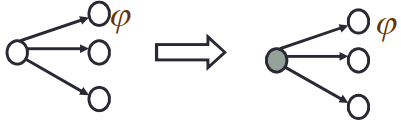
\includegraphics[scale=0.5]{EX.png}
	\centering
	\caption{Exemple EX}
	\label{label-image6}
\end{figure}

\newpage

\subsection{EG}

Voici l'algorithme permetant d'implémenter EG $\varphi$: \\ Tout d'abord, on étiquette les noeuds ayant le label $\varphi$ avec le label EG $\varphi$. Ensuite, et ce tant qu'il n'y a plus de changement, on enlève le label EG $\varphi$ des noeuds n'ayant pas d'enfants avec le label EG $\varphi$. 

\begin{algorithm}[H]
  \caption{Exist Global}\label{euclid}
  \begin{algorithmic}[1]
  \Procedure{EG}{Node $\var{noeud}$, label $\varphi$}
  \State ajouter le label EG$\varphi$ à tous les noeuds ayant le label $\varphi$
  \Do
  \State $\var{SomethingHasChanged} \gets$ False
    \State Enlever le label EG$\varphi$ aux noeuds n'ayant pas d'enfant avec le label EG$\varphi$
    \If {Une modification a eu lieu durant l'étape précédente}
    \State $\var{SomethingHasChanged} \gets$ True
    \EndIf
  \doWhile{$\var{SomethingHasChanged}$}
  \EndProcedure
  \end{algorithmic}
\end{algorithm}

\subsubsection{Exemple d'execution}

Voici la façon dont fonctionne cet algorithme vu sous forme de schéma.

\begin{figure}[!h]
	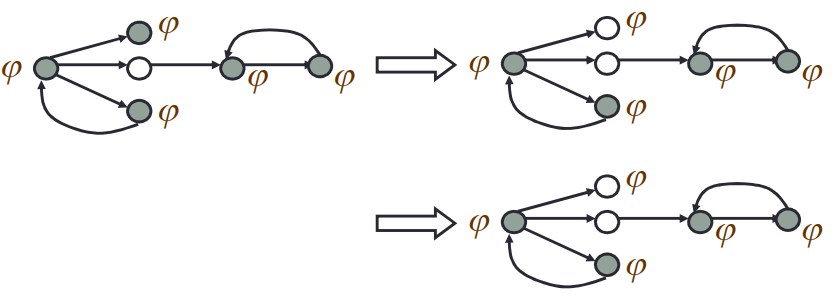
\includegraphics[scale=0.5]{EG.png}
	\centering
	\caption{Exemple EG}
	\label{label-image7}
\end{figure}

\subsection{EU}

Voici l'algorithme afin d'implémenter EU[$\varphi$  U  $\psi$]: \\ En premier lieu, on étiquette avec le label EU[$\varphi$  U  $\psi$] les noeuds ayant le label $\psi$. Ensuite, et ce tant qu'il n'y a pas de changement, on ajoute le label EU[$\varphi$  U  $\psi$] aux noeuds ayant le label $\varphi$ et ayant un enfant avec le label EU[$\varphi$  U  $\psi$].

\begin{algorithm}[H]
  \caption{Exist Union}\label{euclid}
  \begin{algorithmic}[1]
  \Procedure{EU}{Node $\var{noeud}$, label $\varphi$, label $\psi$}
  \State ajouter le label EU[$\varphi$  U  $\psi$] à tous les noeuds ayant le label $\psi$
  \Do
  \State $\var{SomethingHasChanged} \gets$ False
    \State Ajouter le label EU[$\varphi$  U  $\psi$] aux noeuds ayant le label $\varphi$ et ayant un enfant avec le label EU[$\varphi$  U  $\psi$]
    \If {Une modification a eu lieu durant l'étape précédente}
    \State $\var{SomethingHasChanged} \gets$ True
    \EndIf
  \doWhile{$\var{SomethingHasChanged}$}
  \EndProcedure
  \end{algorithmic}
\end{algorithm}

\subsubsection{Exemple d'execution}

Voici la façon dont fonctionne cet algorithme vu sous forme de schéma.

\begin{figure}[!h]
	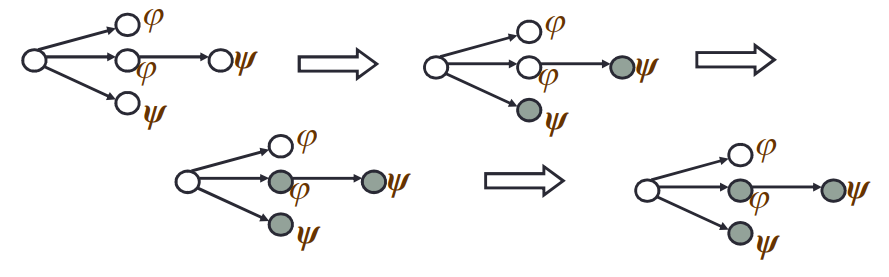
\includegraphics[scale=0.5]{EU.png}
	\centering
	\caption{Exemple EU}
	\label{label-image8}
\end{figure}

\subsection{Autres opérations}

Il est facile de prouver la véracité des relations citées permettant de définir l'ensemble des huit opérations comme étant une combinaison des trois opérations primaires définies plus haut.

\noindent En effet, si nous prenons par exemple la relation "AF $\varphi \Leftrightarrow \lnot$ EG $\lnot \varphi$", celle-ci signifie que "AF $\varphi$" est équivalent à dire qu'il n'existe pas de chemin dans lequel $\varphi$ n'est présent dans aucun des états futures, ce qui est bel et bien équivalent à dire que $\varphi$ apparait dans un état future de chaque chemin.

\noindent Il en va de même pour chacune des opérations restantes. \\ 

\noindent Tous les algorithmes ont été inspirés de publications universitaires tels que \cite{LectureA}, \cite{LectureB}, \cite{LectureC} et \cite{LectureD}

\section{Chapitre 3}
\subsection{Résultats}
Dans le cadre de ce travail, il a été choisi de hardcoder les formules CTL afin de faciliter l'implémentation des algorithmes. Malheureusement, cela a pour conséquence la forte réduction du champs des possibles. En effet, il n'est pas possible d'effectuer d'imbriquations d'opérations telle que "AG AF $\varphi$". \\
\noindent Cependant, il est tout à fait possible d'appliquer les opérations une à une. Ainsi, si on reprend une nouvelle fois notre modèle Kripke de la Figure \ref{label-image3}, et qu'on effectue par exemple "AG fermé", voici ce que l'on obtien : 

\begin{figure}[!h]
	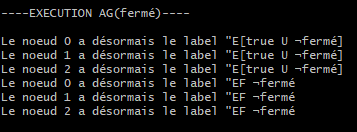
\includegraphics[scale=0.8]{executionExemple.png}
	\centering
	\caption{Exemple d'exécution AG}
	\label{label-image9}
\end{figure}

\noindent Interprétons ce résultat : Comme nous l'avons vu, "AG $\varphi \Leftrightarrow \lnot$ EF $\lnot \varphi$". Afin d'exécuter "AG fermé", il nous faut d'abord effectuer "EF $\lnot$ fermé". Mais nous avons également vu que "EF $\varphi \Leftrightarrow$ E[True U $\varphi$]". Le programme va donc en premier lieu exécuter E[True U $\lnot$ fermé] afin de déterminer les noeuds ayant le label "AF $\lnot$ fermé" et enfin pouvoir déterminer quels noeud présentent le label "AG fermé".\\
\noindent Dans notre cas, nous nous rendons compte qu'aucun état ne présente le label AG fermé. Effectivement, il n'existe pas d'état tel que dans tous les chemins partant de celui-ci, "fermé" apparait dans tous les états futures.\\

\noindent En plus de l'implémentation sur le modèle Kripke, il est également possible d'effectuer ces opérations sur une structure d'arbre dont on a parlé précédemment. Mais il est à noté que la taille de l'arbre ne peut pas être infinie en mémoire et qu'il se peut donc qu'un système présente une erreur sans que l'algorithme ne le détecte. \\

\noindent Le code source est disponnible sur \\ \url{https://github.com/PqMichael/CTL-Model-Checking}

\section{Conclusion}

Nous avons maintenant idée de ce qu'est le Model Checking et de tout ce qu'il permet, en plus de quoi nous avons ajouté notre propre implémentation, même si celle-ci s'avère incomplète. Il serait donc intéressant de continuer celle-ci afin de pouvoir vérifier d'avantage de propriétés sur divers modèles. \\

\noindent Attention cependant, le modèle checking CTL présente un inconvénient : le nombre d'état et variables du système. En effet, l'augmentation de variables dans un système implique une augmentation exponentielle de la taille du modèle, compliquant ainsi la vérification du modèle.
Plusieurs recherches à ce sujet ont déjà été menées (dans \cite{a2} par exemple) et sont encore menées comme dit dans \cite{a1}.\\
D'avantages de problèmes sont cités par \citep{a3}.

\bibliography{references}{}
\bibliographystyle{plain}
\end{document}